\documentclass{article}
\usepackage{tikz,amsmath,amsthm,tkz-graph}
\usetikzlibrary{positioning}
\tikzset{box/.style={draw, thick, text centered, minimum height=0.5cm, minimum width=1cm}}
\tikzset{line/.style={draw, thick, -latex'}}
\title{CSC 226 Problem Set 2 Written Part}
\author{%
	Oliver Tonnesen\\
	V00885732}
\date{October 25, 2018}
\begin{document}
\maketitle
\section{Number of nodes and balance}
	The following sequence of 7 insertions maximizes the number of nodes in a 2--3 tree:
	\[d,b,f,a,c,e,g\]
	The Red-Black tree representation of the 2--3 tree:
	\newline
	\newline
	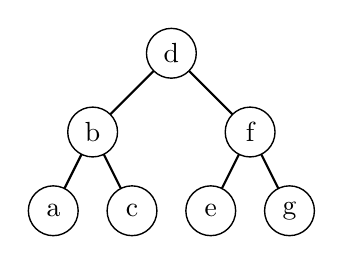
\begin{tikzpicture}
		\Vertex					{d}
		\Vertex[x=-1,y=-1]		{b}
		\Vertex[x=1,y=-1]		{f}
		\Vertex[x=-1.5,y=-2]	{a}
		\Vertex[x=-0.5,y=-2]	{c}
		\Vertex[x=0.5,y=-2]		{e}
		\Vertex[x=1.5,y=-2]		{g}

		\Edge			(d)(b)
		\Edge			(d)(f)
		\Edge			(b)(a)
		\Edge			(b)(c)
		\Edge			(f)(e)
		\Edge			(f)(g)
	\end{tikzpicture}
	\newline
	\newline
	The following sequence of 8 insertions minimizes the number of nodes in a 2--3 tree:
	\[a,c,d,f,g,b,e,h\]
	The Red-Black tree representation of the 2--3 tree:
	\newline
	\newline
	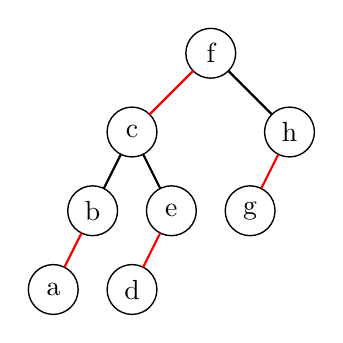
\begin{tikzpicture}
		\Vertex					{f}
		\Vertex[x=-1,y=-1]		{c}
		\Vertex[x=1,y=-1]		{h}
		\Vertex[x=-1.5,y=-2]	{b}
		\Vertex[x=-0.5,y=-2]	{e}
		\Vertex[x=0.5,y=-2]		{g}
		\Vertex[x=-2,y=-3]		{a}
		\Vertex[x=-1,y=-3]		{d}

		\Edge[color=red](f)(c)
		\Edge			(f)(h)
		\Edge			(c)(b)
		\Edge			(c)(e)
		\Edge[color=red](h)(g)
		\Edge[color=red](b)(a)
		\Edge[color=red](e)(d)
	\end{tikzpicture}
	\newline
	\newline
	In general, the larger the number of 3--nodes in a 2--3 tree, the higher the `imbalance'
	of the corresponding Red-Black tree. When a 2--3 tree has only 2--nodes, it is exactly
	the same as its Red-Black tree representation; since a 2--3 tree is always perfectly
	balanced, this Red-Black tree is also perfectly balanced. In a Left-Leaning Red-Black
	representation of a 2--3 tree, the imbalance comes from an abundance of 3--nodes. If the
	2--3 tree has a large number of 3--nodes on a single branch, the corresponding Red-Black
	tree will be very imbalanced due to the red links following the path of the 3--nodes in the
	2--3 tree.
\section{A hybrid MST algorithm}
	Claim: The algorithm constructs the minimum weight spanning tree of $G$.\\
	Proof: [Induction]\\\\
	For the first step, $A=\emptyset$. We know that both Kruskal's and Prim's algorithms
	are correct, so running either initially will not add an edge that does not belong to
	the minimum weight spanning tree, and thus the first step of our hybrid algorithm is
	correct.\\\\
	Suppose there exists some $k$ such that the first $k$ iterations of the algorithm only
	add edges belonging to the minimum weight spanning tree of the graph.\\
	By the $k^{\text{th}}$ iteration of the algorithm, we have a subgraph of the minimum
	weight spanning tree of $G$. We now have the following two cases: the case that our
	constructed subgraph has an even number of edges, and we use a variation of Kruskal's
	algorithm, and the case that our constructed has an odd number of edges, and we use a
	variation of Prim's algorithm. For both cases, we will define a cut that satisfies
	the Cut Property Theorem to prove that the iteration of the algorithm will successfully
	add an edge that does belong to the minimum weight spanning tree of $G$.\\\\
	In the first case, we define $S=\{v\in{V};\exists{u\in{V}},{uv}\in{A}\lor{vu}\in{A}\}$. So
	$S$ contains only vertices that are part of the subgraph of the minimum weight spanning
	tree of $G$ constructed so far by the algorithm. In other words, no vertex in $S$ has an
	edge in $A$ that connects it with a vertex not in $S$. Thus, by the Cut Property
	Theorem, the minimum weight edge crossing the cut $(S,V\setminus{S})$ must be in the
	minimum weight spanning tree of $G$. This is the edge the algorithm now chooses, so this
	step is correct.\\\\
	In the second case, we define $S=\{v\in{V};\text{v is in the randomly selected component}\}$.
	We now define the cut $(S,V\setminus{S})$. By the Cut Property Theorem, the minimum weight
	edge crossing this cut must be in the minimum weight spanning tree of $G$. This is the edge
	the algorithm now chooses, so this step is also correct.\\
	By induction, we have now shown that our hybrid algorithm constructs the minimum weight
	spanning tree of $G$.\qed{}
\section{Uniqueness of MSTs}
	Proof: [Contradiction]
	Suppose $G$ has two minimum weight spanning trees, $A$ and $B$. Consider the minimum weight
	edge $e_1=vu$ that is in $B$ but that is not in $A$, and add it to $A$. Since $A$ was a tree,
	adding an edge to it must create a cycle. $B$ must not contain all of the other	edges in the
	cycle, or it would have originally contained a cycle. So there is an edge $e_2$ in the cycle that
	is not in $B$ but that is in $A$. The edge $e_2$ must have weight greater than that of $e_1$,
	since it is the maximum weight edge in the cycle and the graph contains only edges of unique
	weight. So remove this edge from $A$ and replace it with $e$. $A$ is now a spanning tree of
	$G$ with lower weight. This is a contradiction, since $A$ was defined to be a minimum weight
	spanning tree of $G$, and so $G$ can only have a single minimum weight spanning tree if all
	of its edge weights are distinct.\qed{}
\section*{*Non-distinct edge weights*}
	Claim: Kruskal's algorithm constructs a minimum weight spanning tree of a graph $G=(V,E)$ with
	non-distinct edge weights.\\\\
	We will show that every step of Kruskal's algorithm adds an edge that must belong to a
	minimum weight spanning tree of $G$.\\\\
	Proof: [Induction] Let $A$ be the partially complete spanning tree constructed by Kruskal's
	algorithm. Consider the case when $A=\emptyset$. The algorithm adds the lowest weight edge,
	which must be in the minimum weight spanning tree. \\\\
	Suppose there exists some $k$ such that the first $k$ edges added by the algorithm to $A$
	are elements of a minimum weight spanning tree of $G$.\\\\
	By the $k^{\text{th}}$ addition of an edge to $A$, we have a subgraph of a minimum weight
	spanning tree of $G$. We now define $S=\{v\in{v};\exists{u\in{V}},{uv}\in{A}\lor{vu}\in{A}\}$.
	We see that $S$ contains only vertices that are incident to edges in $A$. So we see that the
	cut $(S,V\setminus{S})$ is crossed by no edges in $A$, and thus satisfies the Cut Property
	Theorem. So the minimum weight edge crossing the cut is contained in the minimum spanning tree.
	Kruskal's algorithm does not add edges that would create a cycle, so the non-distinct edge
	weights will only be picked if they are both the minimum weight and do not create a cycle.\\\\
	By induction, we have now shown that Kruskal's algorithm constructs a minimum weight spanning
	tree of $G$ when $G$ has non-distinct edge weights.\qed{}
\section{Quick-Union with Union-by-Rank}
	Let $Rank(u)$ be the furthest distance from $u$'s root to one of its leaves.\\
	We first note that $Connected$ calls $Find$ twice. Since we know $Find$ takes time proportional
	to $h$, where $h$ is the maximum height of the tree, we know that $Connected$ takes time
	proportional to $2h$. So we aim to prove that $\log{n}$ is an upper bound for $h$, and, by
	extension, for $Connected$.\\
	We first consider what exactly must occur in order for $h$ to increase: a call to $Union(u,v)$
	using Union-by-Rank increases $h$ by one exactly when $Rank(u)$ and $Rank(v)$ are equal.
	Consider WLOG the case where $Rank(u)>Rank(v)$. $h$ remains the same before and after
	the call to $Union(u,v)$, since adding one to $Rank(v)$ is at most equal to $Rank(u)$.
	So conversely when $Rank(u)=Rank(v)$, $Union(u,v)$ increases $h$ by one.\\
	We now consider how to maximize height with minimal nodes in our tree:
	\newline
	\newline
	
\begin{tikzpicture}[black/.style={circle,fill=black,inner sep=0pt,minimum size=2mm},
						red/.style={circle,fill=red,inner sep=0pt,minimum size=2mm},
						blue/.style={circle,fill=blue,inner sep=0pt,minimum size=2mm}]
		\node[red]					(0)	{};
	\end{tikzpicture}
	+
	
\begin{tikzpicture}[black/.style={circle,fill=black,inner sep=0pt,minimum size=2mm},
						red/.style={circle,fill=red,inner sep=0pt,minimum size=2mm},
						blue/.style={circle,fill=blue,inner sep=0pt,minimum size=2mm}]
		\node[blue]									(0)	{};
	\end{tikzpicture}
	=
	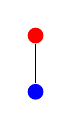
\begin{tikzpicture}[black/.style={circle,fill=black,inner sep=0pt,minimum size=2mm},
						red/.style={circle,fill=red,inner sep=0pt,minimum size=2mm},
						blue/.style={circle,fill=blue,inner sep=0pt,minimum size=2mm}]
		\node[red]											(0)	{};
		\node[blue,node distance=5mm,below=of 0]	(1)	{};

		\draw (0) -- (1);
	\end{tikzpicture}
	\newline
	\newline
	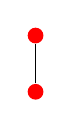
\begin{tikzpicture}[black/.style={circle,fill=black,inner sep=0pt,minimum size=2mm},
						red/.style={circle,fill=red,inner sep=0pt,minimum size=2mm},
						blue/.style={circle,fill=blue,inner sep=0pt,minimum size=2mm}]
		\node[red]								(0)	{};
		\node[red,node distance=5mm,below=of 0]	(1)	{};

		\draw (0) -- (1);
	\end{tikzpicture}
	+
	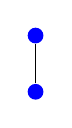
\begin{tikzpicture}[black/.style={circle,fill=black,inner sep=0pt,minimum size=2mm},
						red/.style={circle,fill=red,inner sep=0pt,minimum size=2mm},
						blue/.style={circle,fill=blue,inner sep=0pt,minimum size=2mm}]
		\node[blue]									(0)	{};
		\node[blue,node distance=5mm,below=of 0]	(1)	{};

		\draw (0) -- (1);
	\end{tikzpicture}
	=
	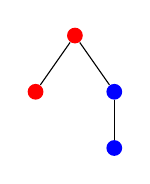
\begin{tikzpicture}[black/.style={circle,fill=black,inner sep=0pt,minimum size=2mm},
						red/.style={circle,fill=red,inner sep=0pt,minimum size=2mm},
						blue/.style={circle,fill=blue,inner sep=0pt,minimum size=2mm}]
		\node[red]											(0)	{};
		\node[red,node distance=5mm,below=of 0,xshift=-5mm]	(1)	{};
		\node[blue,node distance=5mm,below=of 0,xshift=5mm]	(2)	{};
		\node[blue,node distance=5mm,below=of 2]			(3)	{};

		\draw (0) -- (1);
		\draw (0) -- (2);
		\draw (2) -- (3);
	\end{tikzpicture}
	\newline
	\newline
	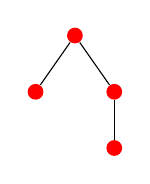
\begin{tikzpicture}[black/.style={circle,fill=black,inner sep=0pt,minimum size=2mm},
						red/.style={circle,fill=red,inner sep=0pt,minimum size=2mm},
						blue/.style={circle,fill=blue,inner sep=0pt,minimum size=2mm}]
		\node[red]											(0)	{};
		\node[red,node distance=5mm,below=of 0,xshift=-5mm]	(1)	{};
		\node[red,node distance=5mm,below=of 0,xshift=5mm]	(2)	{};
		\node[red,node distance=5mm,below=of 2]				(3)	{};

		\draw (0) -- (1);
		\draw (0) -- (2);
		\draw (2) -- (3);
	\end{tikzpicture}
	+
	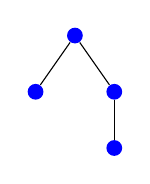
\begin{tikzpicture}[black/.style={circle,fill=black,inner sep=0pt,minimum size=2mm},
						red/.style={circle,fill=red,inner sep=0pt,minimum size=2mm},
						blue/.style={circle,fill=blue,inner sep=0pt,minimum size=2mm}]
		\node[blue]											(0)	{};
		\node[blue,node distance=5mm,below=of 0,xshift=-5mm](1)	{};
		\node[blue,node distance=5mm,below=of 0,xshift=5mm]	(2)	{};
		\node[blue,node distance=5mm,below=of 2]			(3)	{};

		\draw (0) -- (1);
		\draw (0) -- (2);
		\draw (2) -- (3);
	\end{tikzpicture}
	=
	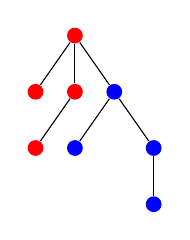
\begin{tikzpicture}[black/.style={circle,fill=black,inner sep=0pt,minimum size=2mm},
						red/.style={circle,fill=red,inner sep=0pt,minimum size=2mm},
						blue/.style={circle,fill=blue,inner sep=0pt,minimum size=2mm}]
		\node[red]											(0)	{};
		\node[red,node distance=5mm,below=of 0,xshift=-5mm]	(1)	{};
		\node[red,node distance=5mm,below=of 0]				(2)	{};
		\node[red,node distance=5mm,below=of 2,xshift=-5mm]	(3)	{};
		\node[blue,node distance=5mm,below=of 0,xshift=5mm]	(10)	{};
		\node[blue,node distance=5mm,below=of 10,xshift=-5mm](11)	{};
		\node[blue,node distance=5mm,below=of 10,xshift=5mm](12)	{};
		\node[blue,node distance=5mm,below=of 12]			(13)	{};

		\draw (0) -- (1);
		\draw (0) -- (2);
		\draw (2) -- (3);
		\draw (0) -- (10);
		\draw (10) -- (11);
		\draw (10) -- (12);
		\draw (12) -- (13);
	\end{tikzpicture}
	\newline
	\newline
	Drawing our the first few trees, the pattern becomes obvious: in order to increase
	$h$, we must at least double the number of nodes. This is due to the fact that we
	our trees must have the same rank in order for $h$ to increase, and beginning with
	two trivial trees allows us to construct the tree with the minimum number of nodes
	that also has height $h$.\\
	So we must at least double our nodes to increase $h$ by one. In other words, if $n$
	is the number of nodes:
	\begin{align*}
		h&=0 \Leftrightarrow n\ge1=2^0\\
		h&=1 \Leftrightarrow n\ge2=2^1\\
		h&=2 \Leftrightarrow n\ge4=2^2\\
		h&=3 \Leftrightarrow n\ge8=2^3\\
		&\quad\quad\vdots\\
		h&=k \Leftrightarrow n\ge2^k\\
	\end{align*}
	So we have, in general,
	\begin{align*}
		n\ge2^h\\
		\log_2{n}\ge{h}\\
		\implies{h\in{O(\log{n})}}
	\end{align*}
	Recall from above that $Connected$ takes time proportional to $2h$, and thus runs in
	time proportional to $O(2h)\in{O(h)}\in{O(\log{n})}$.\qed{}
\end{document}
